\documentclass[sigconf]{acmart}
\usepackage{booktabs}
%\usepackage{booktabs} % For formal tables


% Copyright
%\setcopyright{none}
%\setcopyright{acmcopyright}
%\setcopyright{acmlicensed}
%\setcopyright{rightsretained}
%\setcopyright{usgov}
%\setcopyright{usgovmixed}
%\setcopyright{cagov}
%\setcopyright{cagovmixed}


% DOI
%\acmDOI{10.475/123_4}

% ISBN
%\acmISBN{123-4567-24-567/08/06}

%Conference
%\acmConference[WOODSTOCK'97]{ACM Woodstock conference}{July 1997}{El
%  Paso, Texas USA}
%\acmYear{1997}
%\copyrightyear{2016}


%\acmArticle{4}
%\acmPrice{15.00}

% These commands are optional
%\acmBooktitle{Transactions of the ACM Woodstock conference}
%\editor{Jennifer B. Sartor}
%\editor{Theo D'Hondt}
%\editor{Wolfgang De Meuter}


\begin{document}
\title{Convulaitional Neural Network for Point Cloud Classification}
\subtitle{EEC 289Q - Final Project}

\author{Ahmed Mahmoud}
\orcid{}
\affiliation{%
  \institution{}
  \streetaddress{}
  \city{}
  \state{}
  \postcode{}
}
\email{}

\author{Muhammad Awad}
\affiliation{%
  \institution{}
  \streetaddress{}
  \city{}
  \state{}
  \postcode{}
}
\email{}




\begin{abstract}
\begin{Huge}
TO DO
\end{Huge}
\end{abstract}


\begin{CCSXML}
<ccs2012>
 <concept>
  <concept_id>10010520.10010553.10010562</concept_id>
  <concept_desc>Computer systems organization~Embedded systems</concept_desc>
  <concept_significance>500</concept_significance>
 </concept>
 <concept>
  <concept_id>10010520.10010575.10010755</concept_id>
  <concept_desc>Computer systems organization~Redundancy</concept_desc>
  <concept_significance>300</concept_significance>
 </concept>
 <concept>
  <concept_id>10010520.10010553.10010554</concept_id>
  <concept_desc>Computer systems organization~Robotics</concept_desc>
  <concept_significance>100</concept_significance>
 </concept>
 <concept>
  <concept_id>10003033.10003083.10003095</concept_id>
  <concept_desc>Networks~Network reliability</concept_desc>
  <concept_significance>100</concept_significance>
 </concept>
</ccs2012>
\end{CCSXML}

%\ccsdesc[500]{Computer systems organization~Embedded systems}
%\ccsdesc[300]{Computer systems organization~Redundancy}
%\ccsdesc{Computer systems organization~Robotics}
%\ccsdesc[100]{Networks~Network reliability}


%\keywords{ACM proceedings, \LaTeX, text tagging}


\maketitle

\section{Introduction} 
\subsection{Problem Statement:}

In this project we are trying to classify 3D point cloud. The data set is sets of \emph{models}. Each model is comprised of a set of $n$ data points. A data points is a tuple of 3D coordinates ($x,y,z$) of the point in the space. Figure on the left shows few examples of the data set we have. Each model is associated with a label (for training) shown under the model. 


The data set consists (ModelNet40 \citep{wu20153d}) of 9840 models for training and 2468 models for testing. Our task is to create a CNN model that can train such data set and achieve good accuracy within the test models. 

\begin{figure}[hbt]
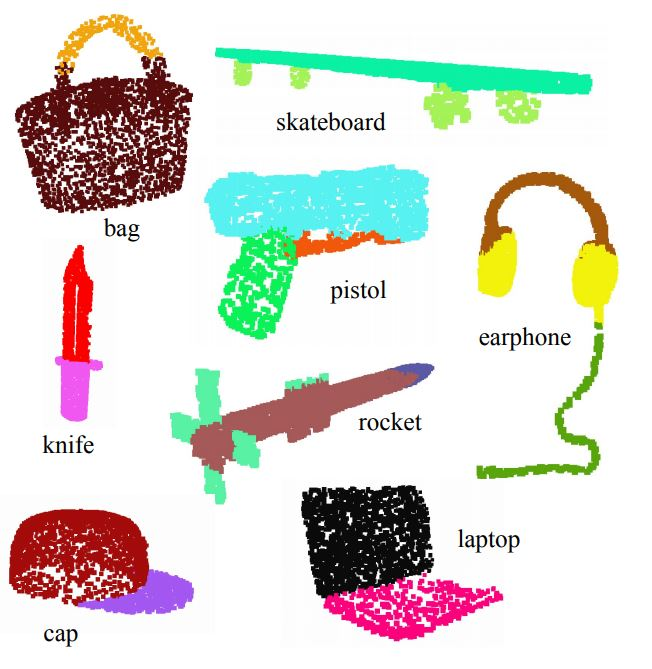
\includegraphics[height=2.5in, width=2.5in]{fig/ex.JPG}
\caption{Example Models (color here are added for visualization only).}
\end{figure}


\subsection{Challenges:}
At first glance the classification looks similar to classifying images which has been investigated thoroughly in the past couple of years. However, we a careful look at the problem and the type of input we have, we can realize the following set of challenges that will influence our model
\paragraph{Irregularity:}
While standard deep neural network models take as input data with regular structure (images of a fixed sizes), point clouds are irregular. This means we have no expectation of the input size (the number of points per models). The reason behind this is that these models either come from scan operations or hand-crafted which can not be constrained to give models of fixed size.

\paragraph{Unordered:} Point positions are continuously distributed in the space and any permutation of their ordering does not change the spatial distribution. The model is read from a file which could store the point in a certain order that is different than other similar models. Thus, associating the feature with the point order could be misleading.
\paragraph{Invariance:} The learned features should be invariant to translation and rotation. Our model should be able to accurately similar models even if they are rotated or shifted. Similar case exists in image where a certain feature could be located anywhere in the image. However, with point cloud in 3D space the problem is augmented as there is a third degree of freedom for translation and rotation. 



\subsection{Previous Work:}
Previous work on point cloud classification using CNN has three main directions:
\paragraph{View-based Methods:}
These methods represents a single model as a collection of 2D views to which standard CNNs used in image classification can be employed directly. View-based appraoches are good match for applications where the input comes from 3D sensor and represented as a range image in which case a single view can be used~\citep{wei2016dense}. 

\paragraph{Volumetric Methods:}
Voxelization is another straightforward way to convert irregular data set to a regular 3D grid over which standard CNN can be applied~\citep{maturana2015voxnet}. Voxelization produces a sparsely-occupied grids and induce quantization artifacts. Cleverer space partition like $k$-d tree can be used to mitigate these problem~\citep{klokov2017escape}.
\paragraph{Direction Methods:}
These methods try to learn from the raw data points without voxelization or alternating the views. It should be expected that these methods to have greater accuracy since we do not manipulate the feature being learned. However, proper model design is challenging due to the challenges been mention earlier. The pioneer work on tackling point cloud learning from the raw data set is PointNet~\citep{pointnet}. PointNet applies a symmetric function to the 3D coordinates in a manner invariant to permutation where every point is treated individually. However, PointNet employs a complex and computationally expensive spatial transformer network to learn the 3D alignment of the points. This is deu to the fact that the feature being learned are global features and no local features are utilized.  
\input{tex/XYZ}
\section{Results}
%exp2
We have conducted different experiments starting with the model shown in Figure~\ref{fig:model1} where we have applied several modification to it to obtain higher performance in terms of accuracy and/or training time. We started without including the point normal information. We observed a large gap between train accuracy and test accuracy indicating an over-fitting. After 200 epochs, the train accuracy was $98\%$ while the test accuracy was $91\%$. Additionally, the model was too slow as it could take upto a day to complete the first 150 epochs on Nvidia Titan V GPU. 

%exp3
The fully connected layers were the bottleneck of our models. The huge number of weights introduced during these two fully connected layers takes up all the computation time. For that, we removed one of them (FC1). Additionally, we decreased the number of channels in each of the first four convolutional layers to be (16, 32, 64, 128). Finally, we reduced the dropout rate to be 0.2 instead of 0.5 (See Figure\ref{fig:model1}). This reduced the training time significantly as it could take 8 hours to train the first 150 epochs. The test accuracy was not affected by these changes; it became $90.07\%$. Surprisingly, this also helped the decreasing the gap between the train accuracy and test accuracy where the train accuracy was $87\%$. 

%exp4
Going to back to how we extracted the features, we could notice that each of the feature layers (labeled as \textbf{EdgeFeatures\_XX} in Figure~\ref{fig:model1} has duplicated information. Each point concatenates its coordinates along with the difference in coordinates with one of its $K$ neighbors. This means that the single point coordinates is being feed to the CNN model $K$ times for each layers. For that, we concatenated the point coordinates only once when $K$ is largest. For other layers, only the local information was feed in. This helped reducing the train time even further. It only took 4 hours to train first 150 epochs. The test accuracy slightly increased to be $90.3\%$ and the train accuracy increased to be $94.5\%$ 

%epx5/exp6/exp7
We now introduce the points normal features and feed it to the CNN model. We do this by replacing \textbf{EdgeFeatures\_10} and \textbf{EdgeFeatures\_30} to be \textbf{NormFeatures\_20} and \textbf{NormFeatures\_40}. That means we take the point and normal information from two set of neighborhood for $K=20$ and $K=40$. We allow concatenation of the point feature and normal feature only for layers with $K=40$. The training time is reduced even further to be 2.5 hours for the first 150 epochs. This is due to the fact the NormFeatures tuple per point is 4 while the EdgeFeatures is 6 which reduced the number of weights. In addition, the train accuracy increased to be $90.6\%$. With further experimentation, we found that we can increase the test accuracy to be $91.5\%$ if we increased the number of channels in the first three convolutional layers to be 64 while increasing the number of channels in the aggregation and fully connected layer to be 512. However, this model take longer to train; more than 5 hours for the first 100 epochs. 
\bibliographystyle{ACM-Reference-Format}
\bibliography{mybib}

\end{document}
